\documentclass[11pt,oneside]{book}

\usepackage[paperheight=297mm,paperwidth=210mm,top=30mm,bottom=30mm,inner=30mm, outer=30mm]{geometry}
\usepackage[utf8]{inputenc}
\usepackage{graphicx}
\usepackage{enumitem}
\usepackage{caption}
\usepackage{subcaption}
\usepackage[nottoc]{tocbibind}
\usepackage{datetime}
\usepackage[colorlinks]{hyperref}
\usepackage{fancyhdr}
\usepackage{setspace}
\usepackage{amsmath}
\usepackage{amssymb}
\usepackage{mathtools}
\usepackage{titlesec}
\usepackage{tocloft}
\usepackage[acronym,nomain,nonumberlist]{glossaries}
\usepackage[table]{xcolor}
\usepackage[toc,page]{appendix}
\usepackage[english]{babel}
\usepackage{etoolbox}

% no new page for each chapter
\makeatletter
\patchcmd{\chapter}{\if@openright\cleardoublepage\else\clearpage\fi}{}{}{}
\makeatother
% no caption prefix
\captionsetup[figure]{labelformat=empty}
% no-indented paragraphs
\setlength{\parindent}{0pt}
% link colors
\hypersetup{citecolor=black, filecolor=black, linkcolor=black, urlcolor=blue}

\newdateformat{monthyeardate}{\monthname[\THEMONTH] \THEYEAR}
\pagestyle{fancy}
\fancyhead{}
\fancyhead[RO]{\nouppercase{\leftmark}}
\renewcommand{\headrulewidth}{0.4pt}

% change chapter title spacing
\titleformat{\chapter}[display]
{\normalfont\huge\bfseries}{\chaptertitlename\ \thechapter}{20pt}{\Huge}
\titlespacing*{\chapter}{0pt}{0pt}{20pt}

%%%%%%%%%%%%%%%%%%%%%%%%%%
%% Document begins here %%
%%%%%%%%%%%%%%%%%%%%%%%%%%
\begin{document}

\pagenumbering{gobble}
\begin{titlepage}
    \begin{center}
        \vspace*{0cm}
        
        \begin{figure}[h]
        \begin{center}
        
\includegraphics[width=.3\columnwidth]{logo.png}
        \end{center}
        \end{figure}
        \vspace*{1cm}
        
        \LARGE
        \textsc{Project Report}
        \vspace{1cm}
                
        \Huge
        \textbf{Graph Attention Networks}
        \vspace{1.5cm}
        
        \LARGE
        Justin Pauckert
        \vspace{1.5cm}
        
        \large 
        Supervised by
        \vspace{.5cm}
        
        \Large 
        Prof. Sebastian Pokutta\\
        Christoph Graczyk
        \vspace{.2cm}
        \setstretch{1.5}
        \vfill
        {\small \monthyeardate\today}
        
        \vspace{1cm}       
        {\Large \textbf{
            Seminar on Discrete Optimization and Machine Learning \\
            Berlin Institute of Technology
            }
        }    
    \end{center}
\end{titlepage} %\pagenumbering{gobble} if we need to remove page numbering

\setstretch{1.0}
\pagenumbering{roman} %Start Roman page numbering
\setstretch{1.5}
\setstretch{1.0}

\clearpage
\newpage

\setstretch{1.0}
\chapter*{Introduction}
\pagenumbering{arabic}
\setstretch{1.25}
\label{chapter:introduction}

As machine learning models find their way in more and more fields of science, allowing them to work with graph data has been a research topic with increasing popularity in recent years. Graphs are commonly used across various fields such as social science (social networks), natural science (protein-protein interactions) and knowledge graphs \cite{zhou2021graph}. In order to allow for this unique data structure, special neural networks have been developed, called \textbf{graph neural networks (GNNs)}. With advancements in the field of deep learning, especially the invention and success of convolutional neural networks, the development of similar methods for graphs suggests itself. In both cases, extracting localized features and composing them to more complex and expressive representations is a major step towards high-performance models for classification and clustering tasks. One way of generalizing convolutions in the graph domain are so-called spatial methods (\cite{hamilton2018inductive}, \cite{monti2016geometric}), where convolutions are defined directly on the graph, operating on groups of spatially close neighbors. Inspired by this idea, \cite{velickovic2018graph} proposed a new architecture to compute node representations by attending over a node's neighbors and assessing their individual importance, called \textbf{graph attention networks (GATs)}. This report covers a short explanation of the proposed idea and discusses some of its benefits in specific applications. Finally, we will give highlight related developments in the field, including concerns over prevalent data sets used for benchmarks and limitations of architectures like GATs.
\\~\\


\setstretch{1.0}
\chapter*{GAT Architecture}
\setstretch{1.25}
\label{chapter:GAT Architecture}

Graph attention networks are build by stacking graph attentional layers, which we will briefly explain in this section, closely following \cite{velickovic2018graph}. The input of a layer is a set of node features, $h = \{h_1,...,h_N\}, h_i \in \mathbb{R}^F$, where $N$ is the number of nodes and $F$ the number of features in each node. The layer produces a new feature representation $h_i' \in \mathbb{R}^{F'}$ for each node $h_i$, possibly of different cardinality $F'$. To that end, a learnable weight matrix $\mathbf{W} \in \mathbb{R}^{F' \times F}$ and a shared attention mechanism $a: \mathbb{R}^{F'} \times \mathbb{R}^{F'} \rightarrow \mathbb{R}$ are introduced. The importance of a node's neighbor, called \textit{attention coefficient}, is then computed as $a(\mathbf{W}h_i, \mathbf{W}h_j)$. Denoting the normalized coefficients as $\alpha_{ij}$, the hidden state of a node $h_i$ can then be obtained by
\begin{align*}
    h_i' = \sigma(\sum_{j \in \mathcal{N}_i} \alpha_{ij}\mathbf{W}h_j)
\end{align*}
where $\mathcal{N}_i$ is the set of indices for neighbors of $h_i$ and $\sigma$ a nonlinear function. This process can be initiated multiple times, resulting in multiple attention mechanisms. This popular method is called \textit{multi-head attention} and was adapted from \cite{vaswani2017attention}. The resulting features can then be concatenated or averaged to improve the models performance  as illustrated in Figure \ref{fig:multi-head}.

\begin{figure}[h]
    \centering
    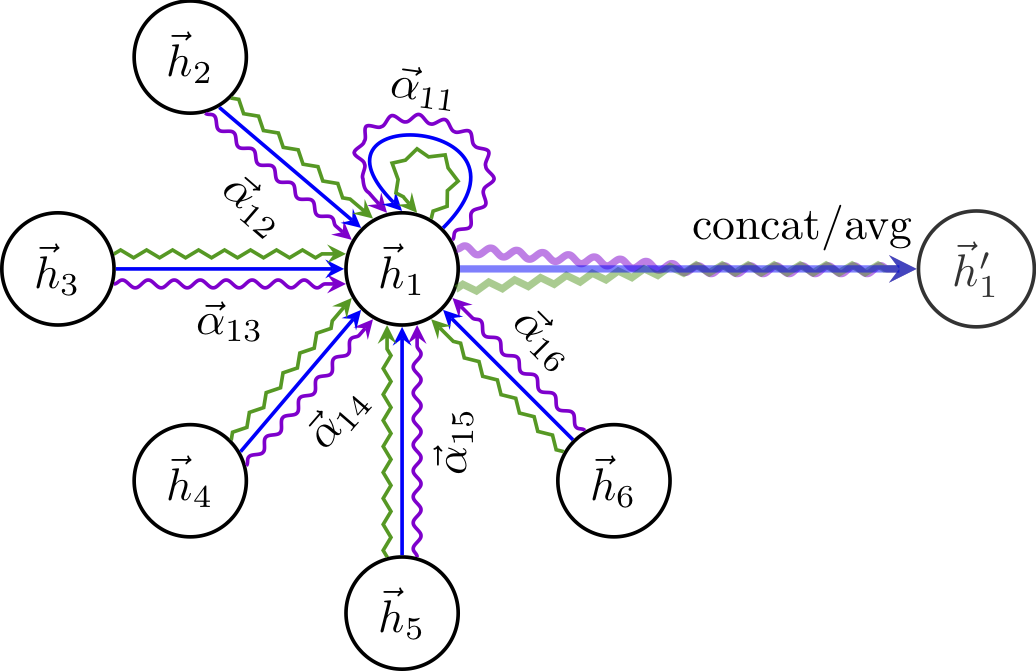
\includegraphics[width=0.5\textwidth]{img/multi_head.png}
    \caption{Multi-head attention with three heads by node $h_1$. \cite{velickovic2018graph}}
    \label{fig:multi-head}
\end{figure}
Allthough this architexture has similarities with prior methods, it solves several issues with its flexibility. We will refer to the original paper for more details but mention two desirable properties that will be important for the subsequent chapters. 

\begin{itemize}[leftmargin=*]
    \item Assigning different importances to nodes of the same neighborhood enables a leap in complexity when compared to graph convolutional networks (GCNs). Furthermore, analyzing the learned attention weights may improve \textbf{explainability} of the model.
    \item Since attention mechanism and feature weight matrix are applied in a shared manner, a trained GAT can be applied to \textbf{inductive} tasks. That is, they can be evaluated on graphs that were completely unseen during training. Many previous approaches depended on upfront access to the whole graph, making them unfeasible for such tasks. 
    \bigskip
\end{itemize}



\setstretch{1.0}
\chapter*{Applications}
\setstretch{1.25}
\label{chapter:applications}

To demonstrate the impact of GATs, we will present two examples for their applications. The first one was developed in collaboration with one of the involved authors shortly after the original paper was published. Then, a fairly recent publication will highlight the relevance of the architecture to this day.

\section*{GATs for Brain Mesh Segmentation}
In \cite{Cucurull2018ConvolutionalNN}, both GCNs and GATs were cutting edge technologies that were assessed against previous mesh parcellation models. Reconstructions of the cortical surface were represented in a graph which had to be divided into areas. Nodes correspond to locations on the brain surface, their features included cortical thickness, curvature and functional connectivity.

The authors considered three kinds of information the models could use: \textit{neighborhood information}, \textit{node features} and \textit{global information}, that is, access to feature information from all the nodes.
Previous approaches for this task were unable to exploit all three kinds of information and were therefor limited in their complexity. Alongside GCNs, GATs outperformed all state-of-the-art models, showing the importance of utilizing the mesh structure in the data. Furthermore, the authors showed that dynamic attention mechanisms actually improve performance when compared to a constant attention for all neighbors.

\begin{figure}[h]
    \centering
    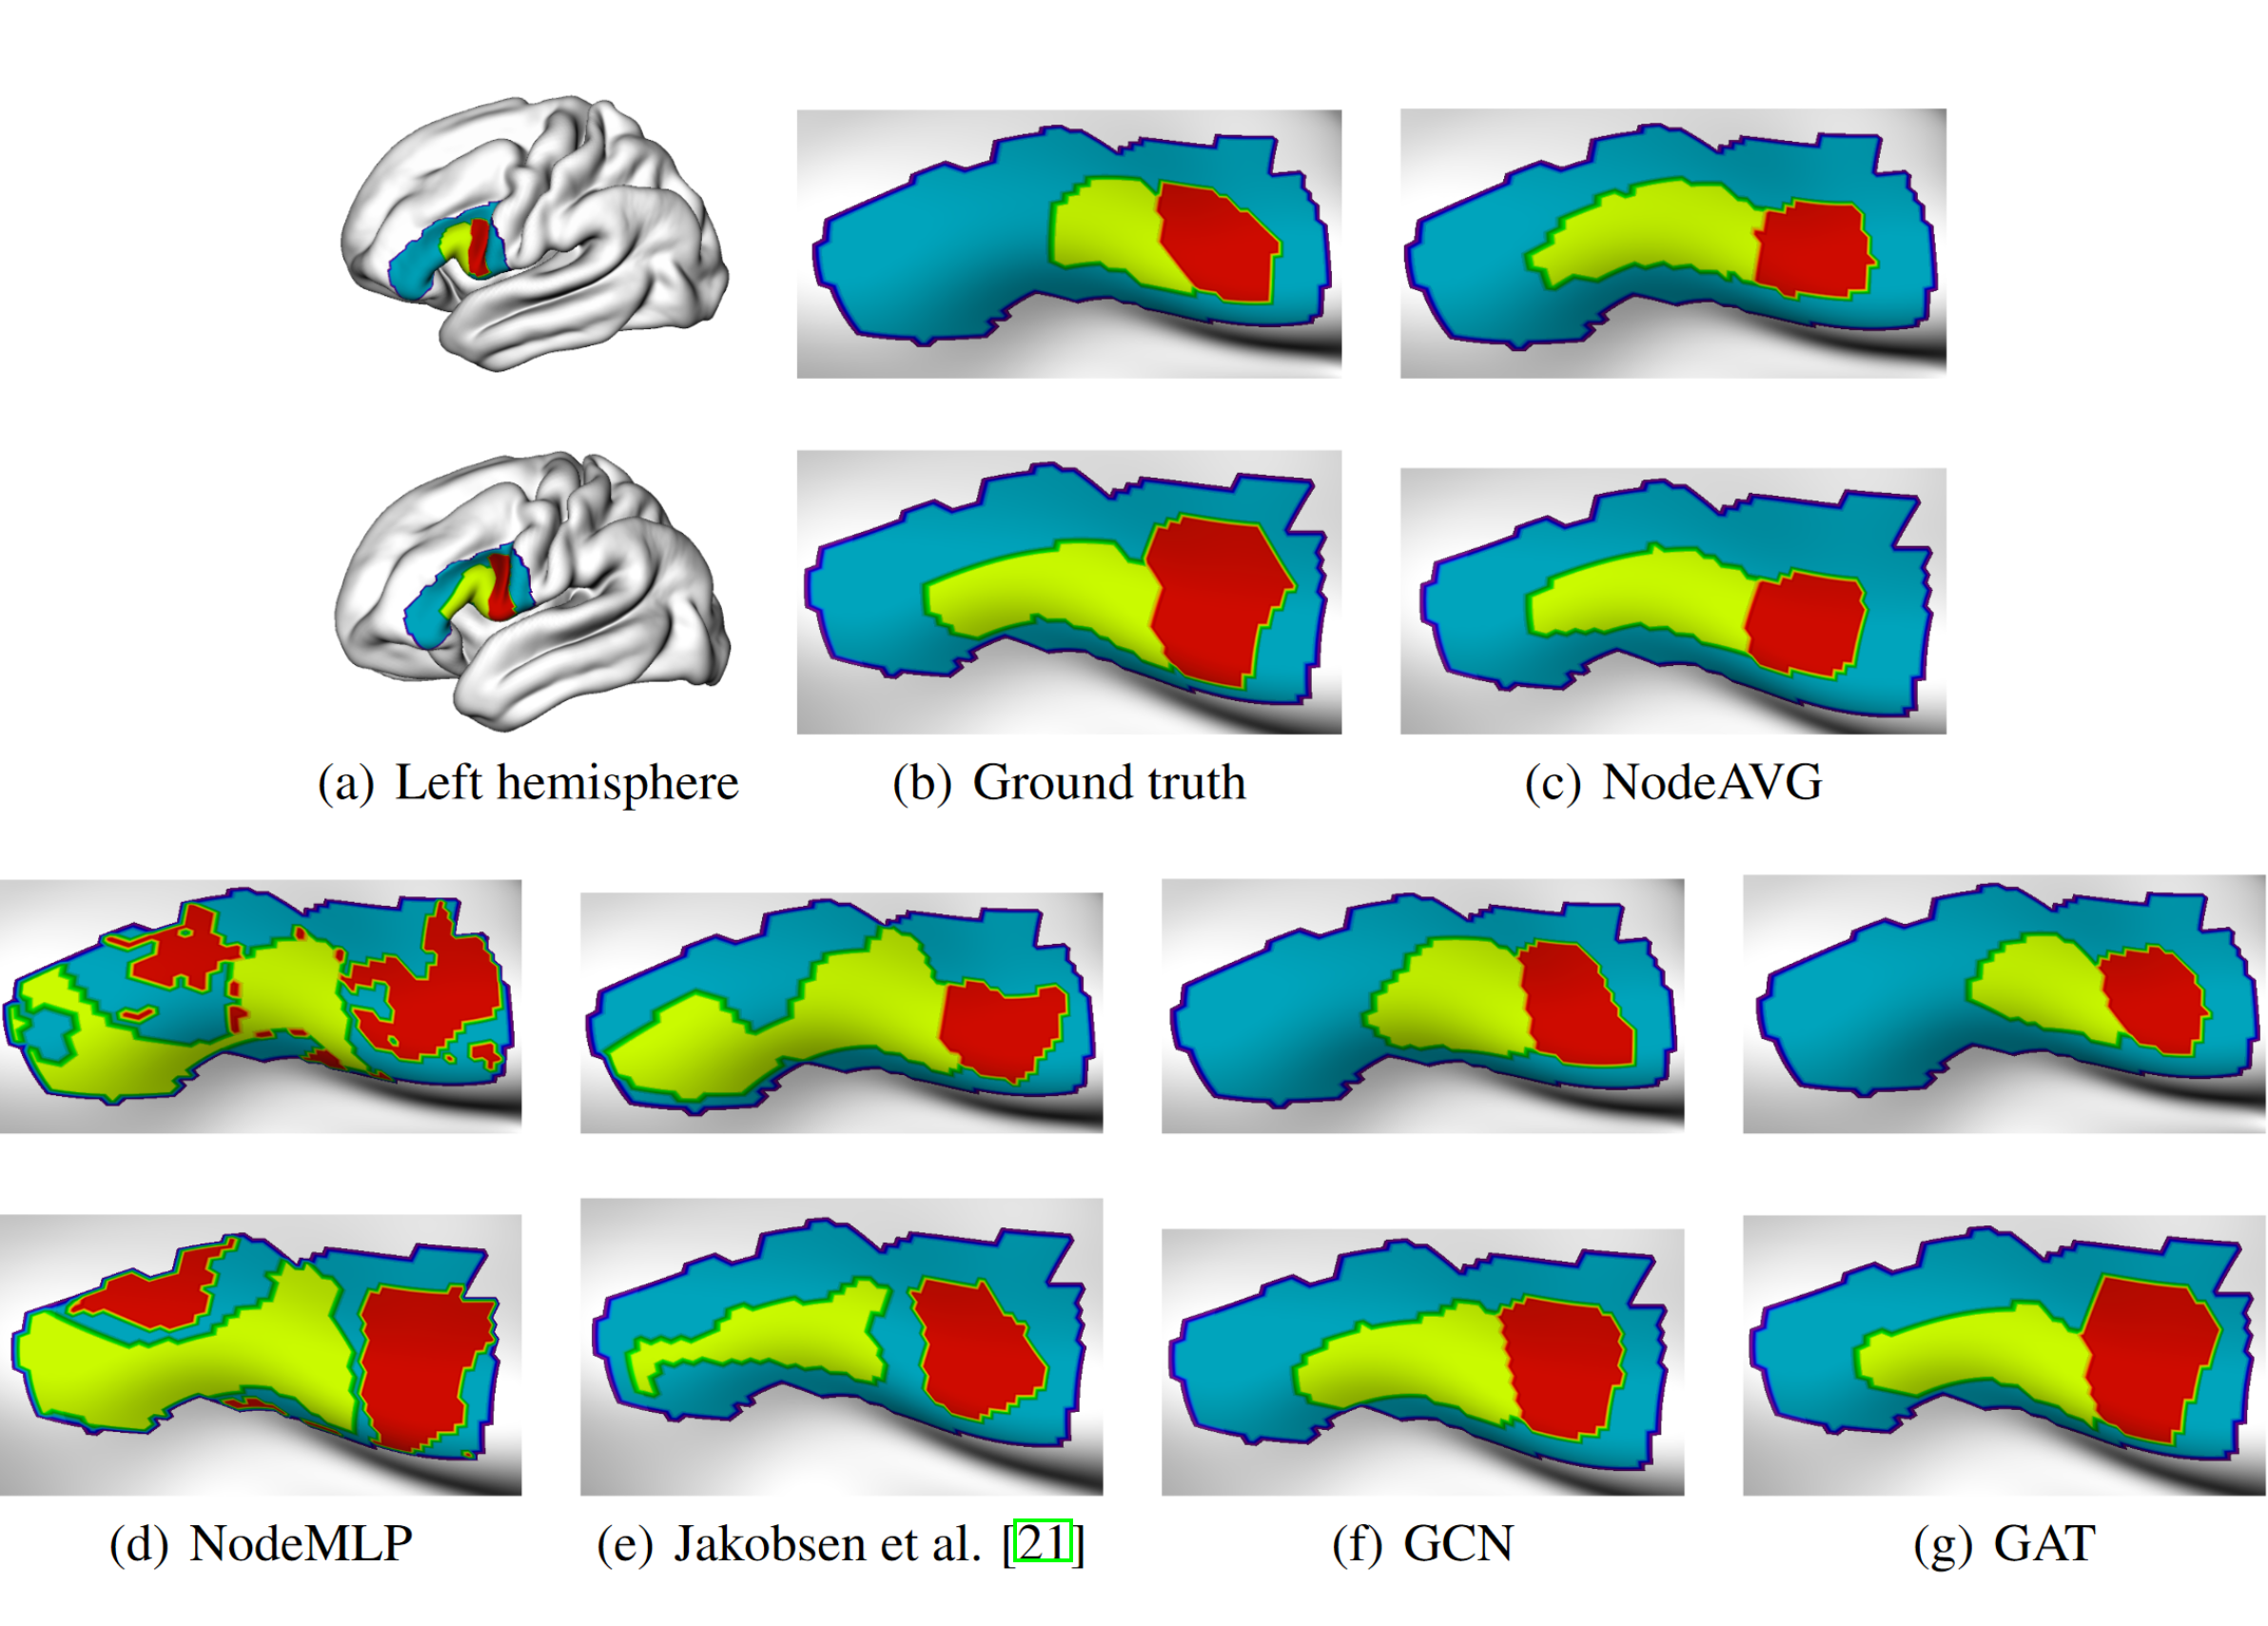
\includegraphics[width=0.75\textwidth]{img/brain_mesh.PNG}
    \caption{Qualitative area parcellation results for two test set subjects. \cite{Cucurull2018ConvolutionalNN}}
\end{figure}

In conclusion, this application demonstrated the potential of GNNs and their applicability to real-world problems. GATs showed promising results, raising hopes for applications in other areas. As we will see later on, this assessment is still up to date and in-line with recent benchmarks.\bigskip

\section*{Improving Explainability through Attention Mechanisms}

Visual Question Answering (VQA) is an important task to build systems that better understand the relationship between vision and language by learning to answer questions about an image. The TextVQA dataset (see \cite{singh2019vqa}) includes image-question pairs that require models to read text in images and answer questions accordingly.

A recent publication by \cite{rao2021look} proposes a model that is able to generate explanations for its answers. These are "consistent with human interpretation, help justify the models' decision and provide useful insights to help diagnose an incorrect prediction". To that end, they build a graph to encode the relatoinship between objects and text. A GAT is then used to variably weigh an object's adjacent text nodes based on relevancy. The attention weights can be visualized as a heat map, highlighting the position of text tokens that were considered important.\medskip

\begin{figure}[h]
    \centering
    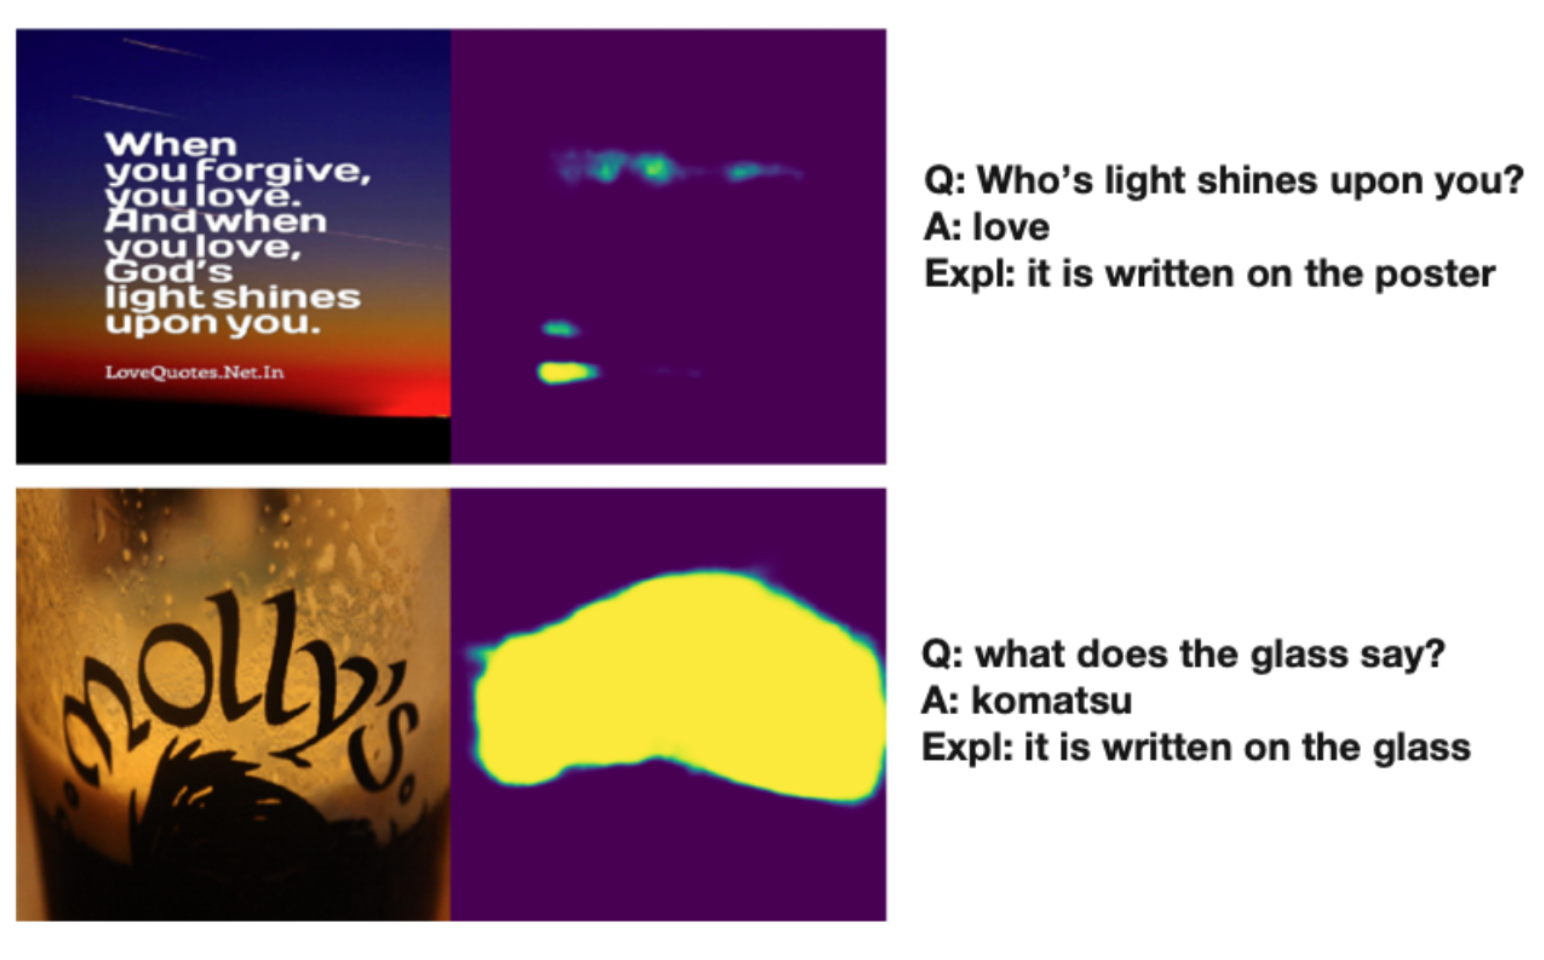
\includegraphics[width=0.75\textwidth]{img/text_3.PNG}
    \caption{Attention weights help explain incorrect decisions. In the first image, the model pays attention to the wrong text tokens. For the second image attention is where it needs to be but the OCR engine fails to read the text correctly. \cite{rao2021look}}
    \medskip
\end{figure}

Allthough there are multiple components to this model, it shows that attention weights can help explain its answers. Therefor, this paper is evidence for the claim about increased interpretability through analysis of attention weights made in \cite{velickovic2018graph}. Once more, it is shown that GATs are still used today and remain an important tool in the graph neural network domain. \bigskip

\setstretch{1.0}
\chapter*{Benchmarking GNNs}
\setstretch{1.25}
\label{chapter:related_work}

benchmarks in Question
depth of GNNs
the road ahead?
 \\

\setstretch{1.0}
\chapter*{Going deep with GNNs}
\setstretch{1.25}
\label{chapter:related_work}

benchmarks in Question
depth of GNNs
the road ahead?
 \\ 

\newpage
\setstretch{1.0}
\bibliographystyle{apalike}
\renewcommand\bibname{References}

\bibliography{references} %copy all references to references.bib file


\end{document}